




In \cite{Verendel_2009} Verendel finds 4 distinct validation methods used across the 90 security metrics papers surveyed: hypothetical, empirical, simulation, and theoretical. The author adds the caveat that no attempt was made to verify the quality of results, only to describe the methods used in each paper to substantiate the findings. In this section we propose a method for validating security metrics through empirical means.

In general, a metric should be both reliable and valid, where reliability refers to the consistency of values across repeated measurements, and validity concerns the accuracy of those values. There is currently no \textit{unit} reference for a security property which we can use for establishing the accuracy of our security metrics. We can, however, examine the behaviour of a metric relative to a given system by manipulating relevant aspects of that system while holding the other properties constant. For example, we can assign vulnerabilities to the small enterprise network shown in Figure \ref{fig:refnet_small}. For metrics that are influenced by the vulnerability score (such as CVSS based metrics), we can fix the weights of these vulnerabilities in the range of possible scores (0.0 to 10.0 in the case of CVSS). This would produce the lower and upper bound for that metric on this specific configuration of system configuration and vulnerability assignment. Similarly, we can alter properties such as the effects of a successful exploit (remote code execution, privilege escalation, etc), the placement and quantity of vulnerabilities, the underlying platform/operating system/applications, connectivity and topology, and so on. By capturing the measured values of controlled alterations to a system, we begin to understand how that metric behaves on the given system. Observing how multiple metrics behave under the same alterations allows us to compare their relative performance without an absolute point of reference. Furthermore, we can extend this analysis from a simple enterprise network to any number of use cases by supplying input adaptors for topology generators such as BRITE\cite{Medina_Lakhina_Matta_Byers_2001} or simulators like SSFNet\cite{Cowie_Ogielski_Nicol_2002} and Mininet\cite{Lantz_Heller_McKeown_2010}. Figure \ref{fig:refnets} shows an example reference set of 3 network topologies of increasing size and complexity. The first represents the type of example network commonly referenced in the literature to demonstrate a newly proposed metric, and the other two were selected from the gallery of publicly available SSFNet topologies and are described by an easy to parse domain specific language. By including systems at different scales, we are able to determine if a metric's performance depends on the size and complexity of the system under test. Intuitively, we would expect the temperature of 1 liter of boiling water to be the same as 1000 liters of boiling water, so testing against systems of varying size allows us to verify this hypothesis.

\begin{figure*}
    \centering
    \begin{subfigure}[t]{0.3\textwidth}
        % \centering
        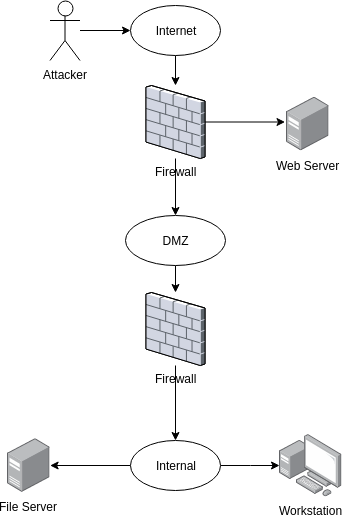
\includegraphics[width=\linewidth]{resource/img/ch_automation/from_ares_paper/net_small.png} 
        \caption{Small-sized network\cite{Ou_Appel_2005}} 
        \label{fig:refnet_small}
    \end{subfigure}
          \begin{subfigure}[t]{0.33\textwidth}
        \centering
        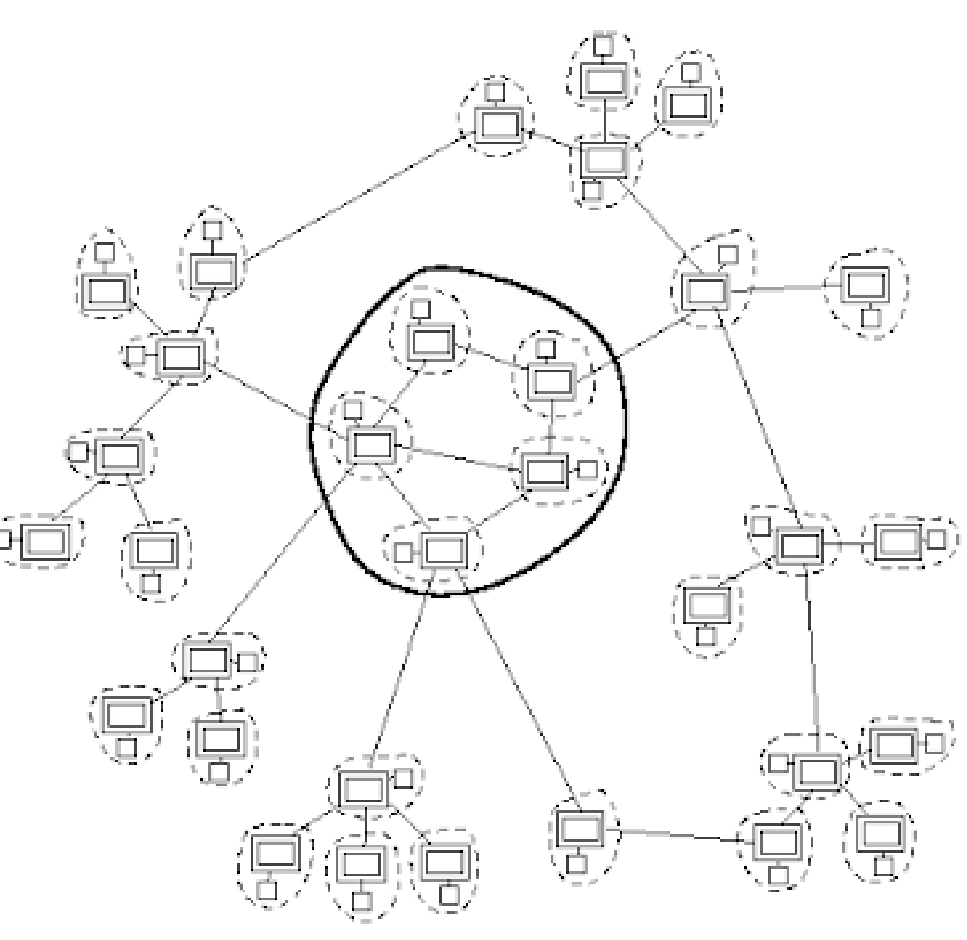
\includegraphics[width=\linewidth]{resource/img/ch_automation/from_ares_paper/net_med_2.png}
        \caption{Medium-sized network\cite{Cowie_Ogielski_Nicol_2002}}
        \label{fig:refnet_med}
    \end{subfigure}
     \begin{subfigure}[t]{0.3\textwidth}
        \centering
        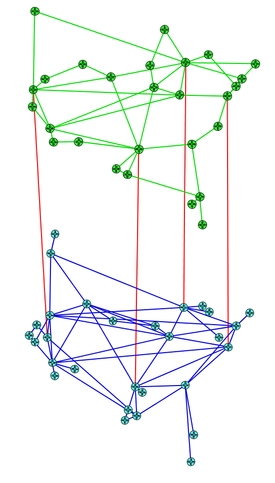
\includegraphics[width=\linewidth]{resource/img/ch_automation/from_ares_paper/net_large.png}
        \caption{Large-sized  network\cite{Cowie_Ogielski_Nicol_2002}}
        \label{fig:refnet_large}
    \end{subfigure}
    \hfill
    \caption{Different Sized Reference Networks}
    \label{fig:refnets}
\end{figure*}

If we consider a security metric as a measurement instrument, then we can validate the metric by characterizing its behavior against a reference set. Some security metric properties we might consider for validation can be taken directly from the field of measurement theory. In addition to accuracy and precision, Morris\cite{Morris_2001} describes several performance characteristics of measurement instruments that we may adapt to our validation of security metrics:

\textbf{Monotonicity}: Does the measured value always increase or always decrease with respect to each improvement in security.

\textbf{Linearity}: For security levels $s_1$ and $s_2$ and incremental security improvement $i$, is the difference between $(s_1,i)$ the same as $(s_2,i)$?

\textbf{Range}: What are the upper and lower bounds that a metric will assume for a specific model?

\textbf{Precision}: Does the metric report the same value for repeated measurements of the same quantity? This is of particular interest in probabilistic metrics. 

Analogues to other standard instrument performance measures - threshold, resolution, sensitivity to disturbance, etc - can be adapted to evaluate a security metric against our reference networks as well, and it is still to be determined which characteristics of static measurement instruments are required for their security related counterparts. 
